The last prototype developed was TRITIUM-IFIC-2, shown in Figure \ref{fig:TritiumIFIC2}. This prototype, built in the IFIC workshop, consists of $800$ uncladded BCF-12 scintillating fibres of $200~\mm$ length and $1~\mm$ diameter placed inside a cylindrical PTFE vessel shown in Figure \ref{fig:Tritium-IFIC2_vessels}. The internal length and diameter of the PTFE vessel are $210~\mm$ and $36~\mm$, respectively. The number of fibres used is larger than for the Aveiro prototype but they are contained in a smaller volume. The scintillating fibres are tightly stacked but allowing water to flow between them. The fibres were cleaved, polished and cleaned with the conditioning processes described in section \ref{sec:CharacterizationScintillatingFibers}.Two $5~\mm$ thick PMMA windows allow to read the scintillation light out as in Tritium-Aveiro. 
\begin{figure}[h]
\centering
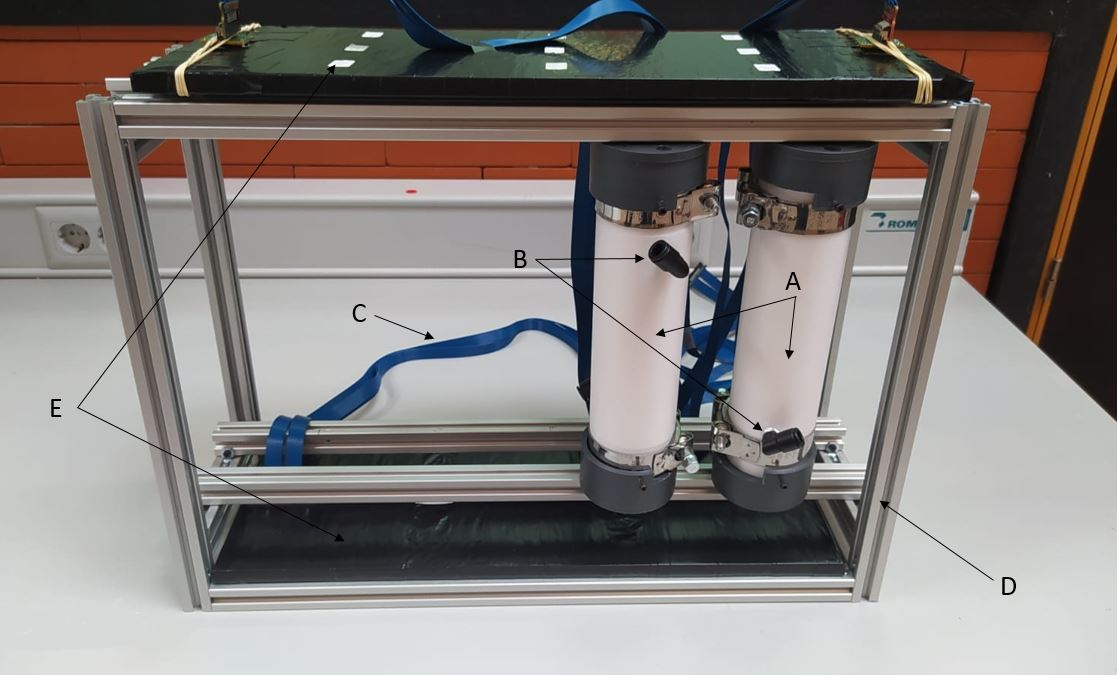
\includegraphics[scale=0.4]{5Prototypes/53FinalPrototypes/532TritiumIFIC2/Tritium_IFIC_2_full_module.jpg}
\caption{(A) TRITIUM-IFIC-2 prototype, (B) water inlet/outlet, (C) PETsys flat wires, (D) the metallic structure and (E) active veto.\label{fig:TritiumIFIC2}}
\end{figure}
\begin{figure}
\centering
    \begin{subfigure}[b]{0.45\textwidth}
    \centering
    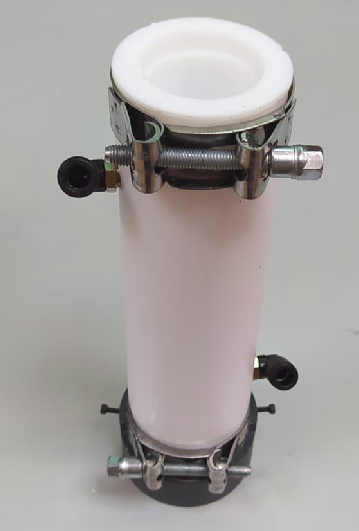
\includegraphics[width=\textwidth]{5Prototypes/53FinalPrototypes/532TritiumIFIC2/Tritium_IFIC_2_vessel1.png}  
    \caption{\label{subfig:Tritium_IFIC_2_vessel}}
    \end{subfigure}
    \hfill
    \begin{subfigure}[b]{0.4\textwidth}
    \centering
    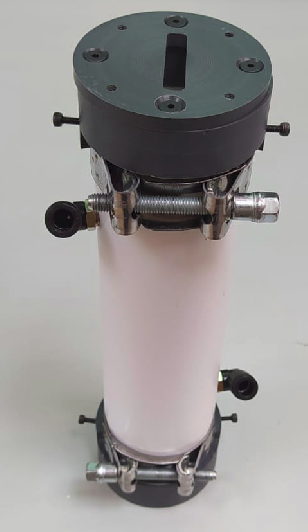
\includegraphics[width=\textwidth]{5Prototypes/53FinalPrototypes/532TritiumIFIC2/Tritium_IFIC_2_vessel2.png}  
    \caption{\label{subfig:TritiumIFIC2_vessel_with_PVC_caps}}
    \end{subfigure}
 \caption{a) TRITIUM-IFIC-2 PTFE vessel. b) TRITIUM-IFIC-2 PTFE vessel with two PVC caps that provide a light-tight environment for the SiPM arrays.}
 \label{fig:Tritium-IFIC2_vessels}
\end{figure}
The windows thickness is enough to seal the vessel since the detector works at very low water pressure. PMMA was chosen for its optical properties, especially its transmission coefficient which was measured at ICMOL and it is plotted in Figure \ref{fig:PMMATransmissionSpectrum}. This transmission coefficient is approximately $95\%$ at the working wavelength ($435~\nm$). Two clamps keep the prototype sealed as in TRITIUM-Aveiro.
\begin{figure}[h]
\centering
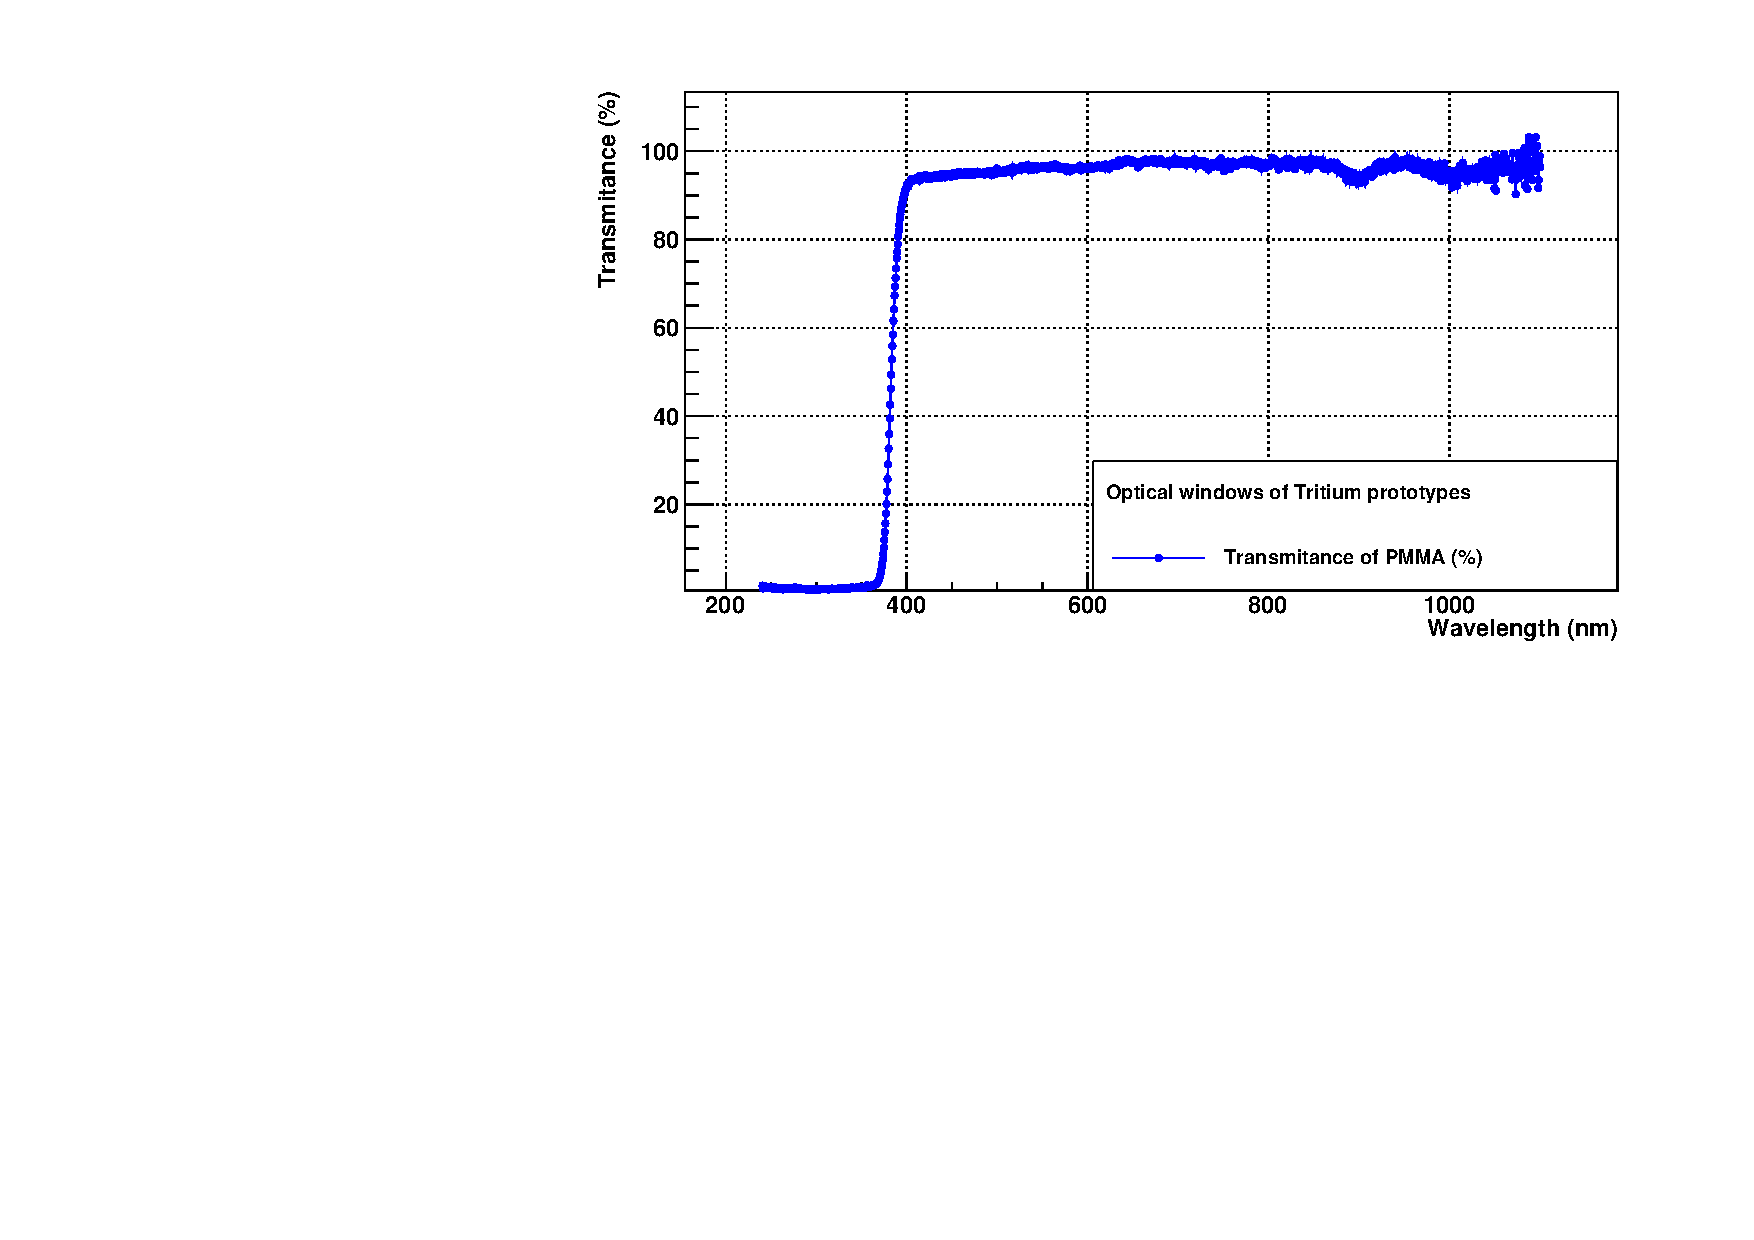
\includegraphics[scale=0.75]{5Prototypes/53FinalPrototypes/532TritiumIFIC2/TransmissionSpectrumPMMA_cut_at_low_energy.pdf}
\caption{Light transmission spectrum of a $5~\mm$ thick PMMA plate, measured at ICMOL. \label{fig:PMMATransmissionSpectrum}}
\end{figure}	
A water inlet/outlet was implemented in the PTFE vessel to allow a constant water flow. 

Two R8520-460 Hamamatsu PMTs \cite{DataSheetPMTs} were used. Measurements with SiPM arrays controlled by PETsys were also performed. PETsys has a graphical user interface that allows to remote control the different input and ouput options such as SiPM arrays bias voltage, thresholds, etc., via a computer terminal. A picture of the GUI is shown in Figure \ref{fig:GUI_PETSYS}.
\begin{figure}[h]
\centering
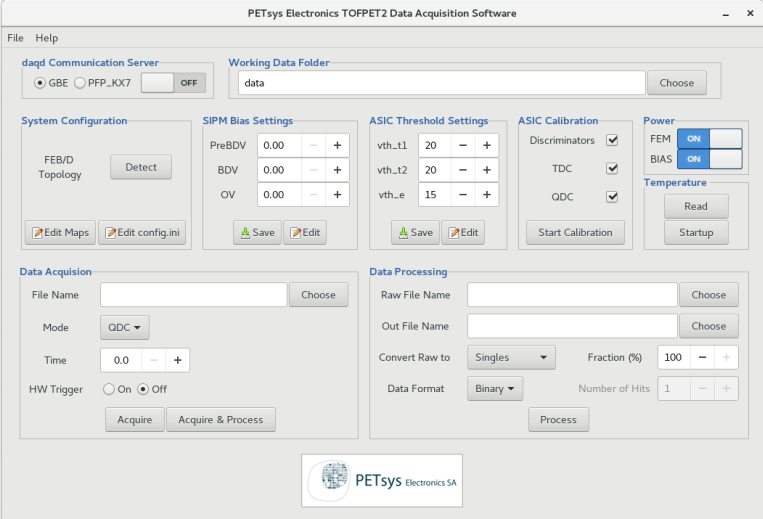
\includegraphics[scale=0.5]{5Prototypes/53FinalPrototypes/532TritiumIFIC2/GUI_PETSYS.png}
\caption{Graphical user interface of PETsys.\label{fig:GUI_PETSYS}}
\end{figure} 

An aluminium structure was built to accommodate up to 10 TRITIUM-IFIC-2 modules and two cosmic vetos, shown in Figure \ref{fig:TritiumIFIC2}. The available space inside the lead shield in Arrocampo site could lodge up to 5 structures. This means that the final TRITIUM monitor could be composed of up to 50 TRITIUM-IFIC-2 modules and 5 different cosmic vetos.

Two identical TRITIUM-IFIC-2 prototypes were built. One was filled with pure water and the second with a tritium liquid source to measuring the background and the signal, respectively. The water volume in both cases was $82~\milli\liter$ (uncertainty of $0.05\%$). The activity of the tritium source employed was $10~\kilo\becquerel/\liter$ (uncertainty of $2.24\%$). The signal and background energy spectra are shown in Figure \ref{fig:EnergySpectraTRITIUMIFIC2}. The energy spectrum of tritium was obtained by substracting the background from the signal spectrum. The rates obtained from these three spectra are given in Table \ref{tab:CountsPerSecondTRITIUMIFIC2}. 

\begin{figure}
\centering
    \begin{subfigure}[b]{0.9\textwidth}
    \centering
    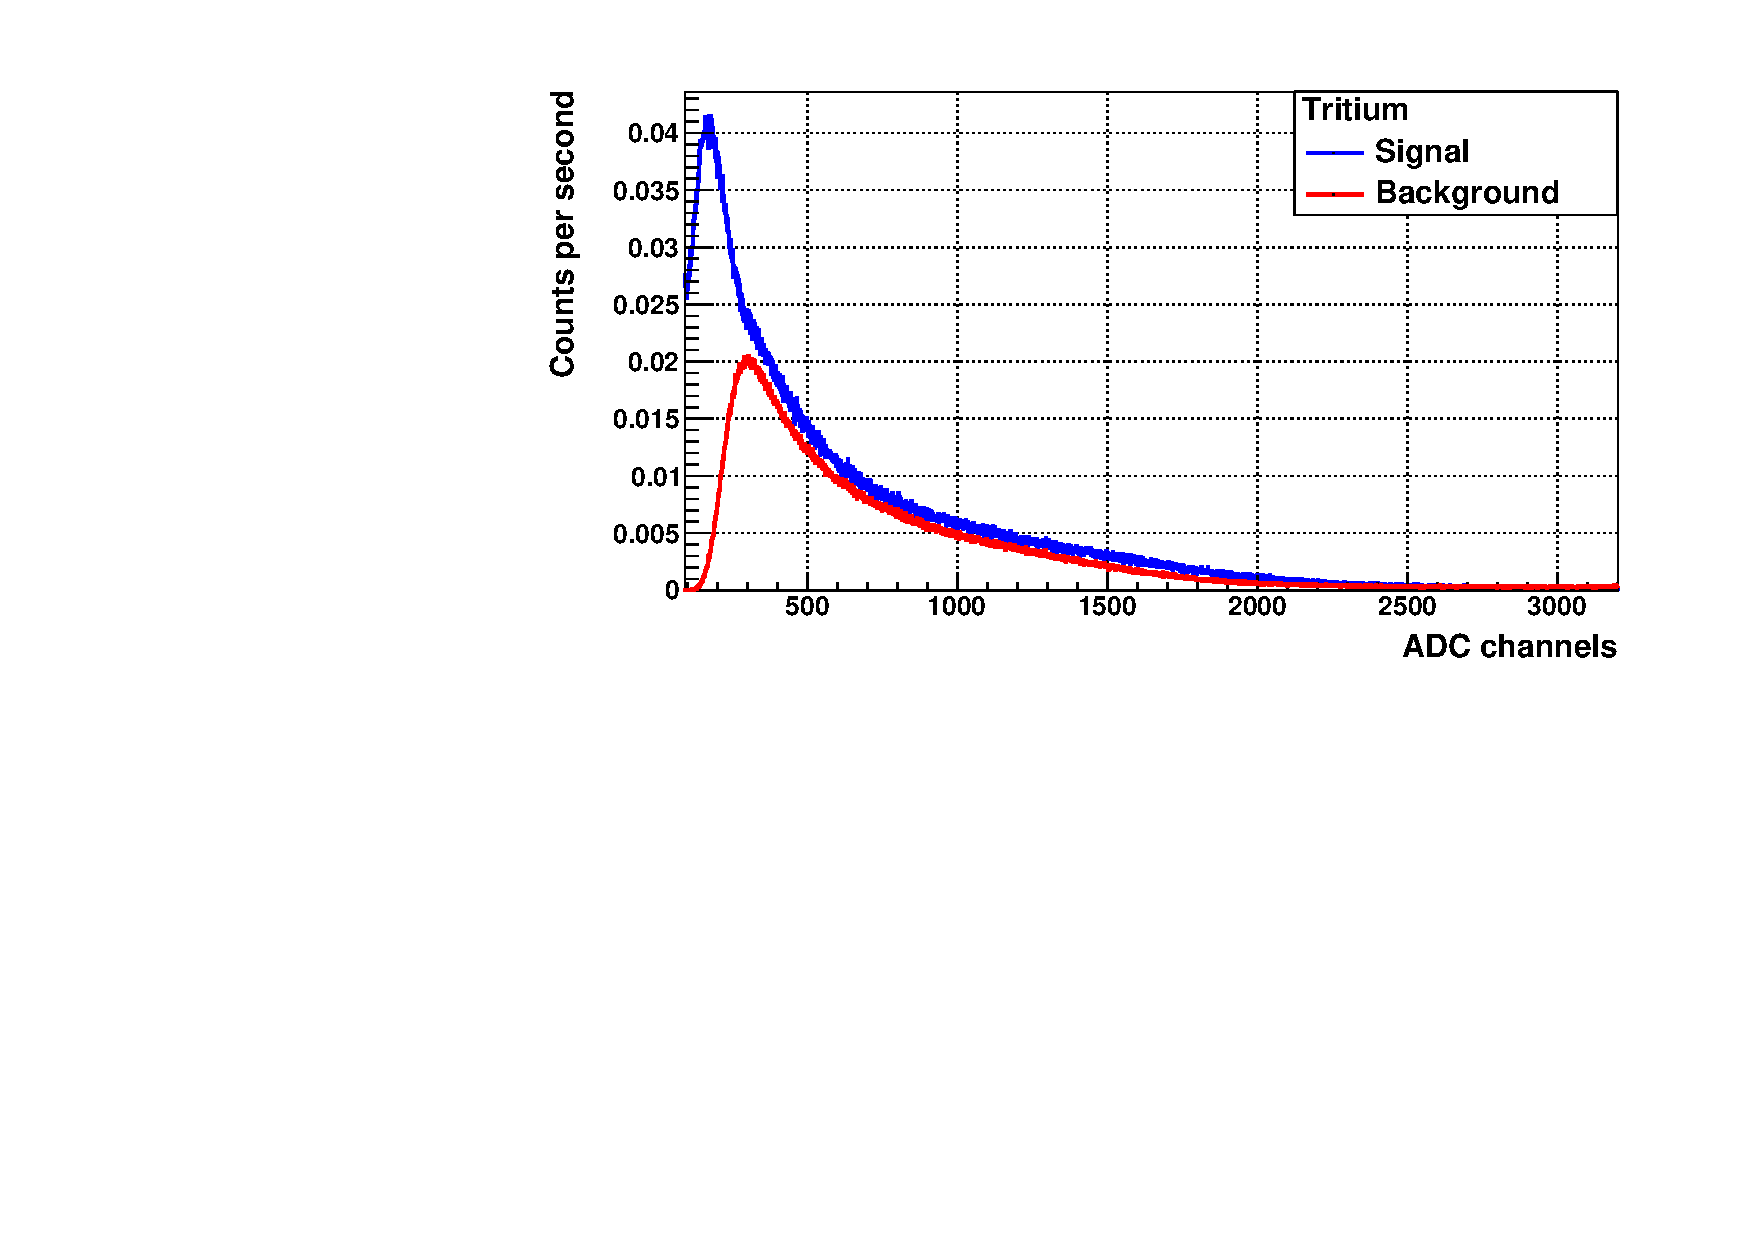
\includegraphics[width=\textwidth]{5Prototypes/53FinalPrototypes/532TritiumIFIC2/TritiumIFIC2SignalsHigherZOOM_NP.pdf}  
    \caption{\label{subfig:SignalBackgroundEnergySpectraTritiumIFIC2}}
    \end{subfigure}
    \hfill
    \begin{subfigure}[b]{0.9\textwidth}
    \centering
    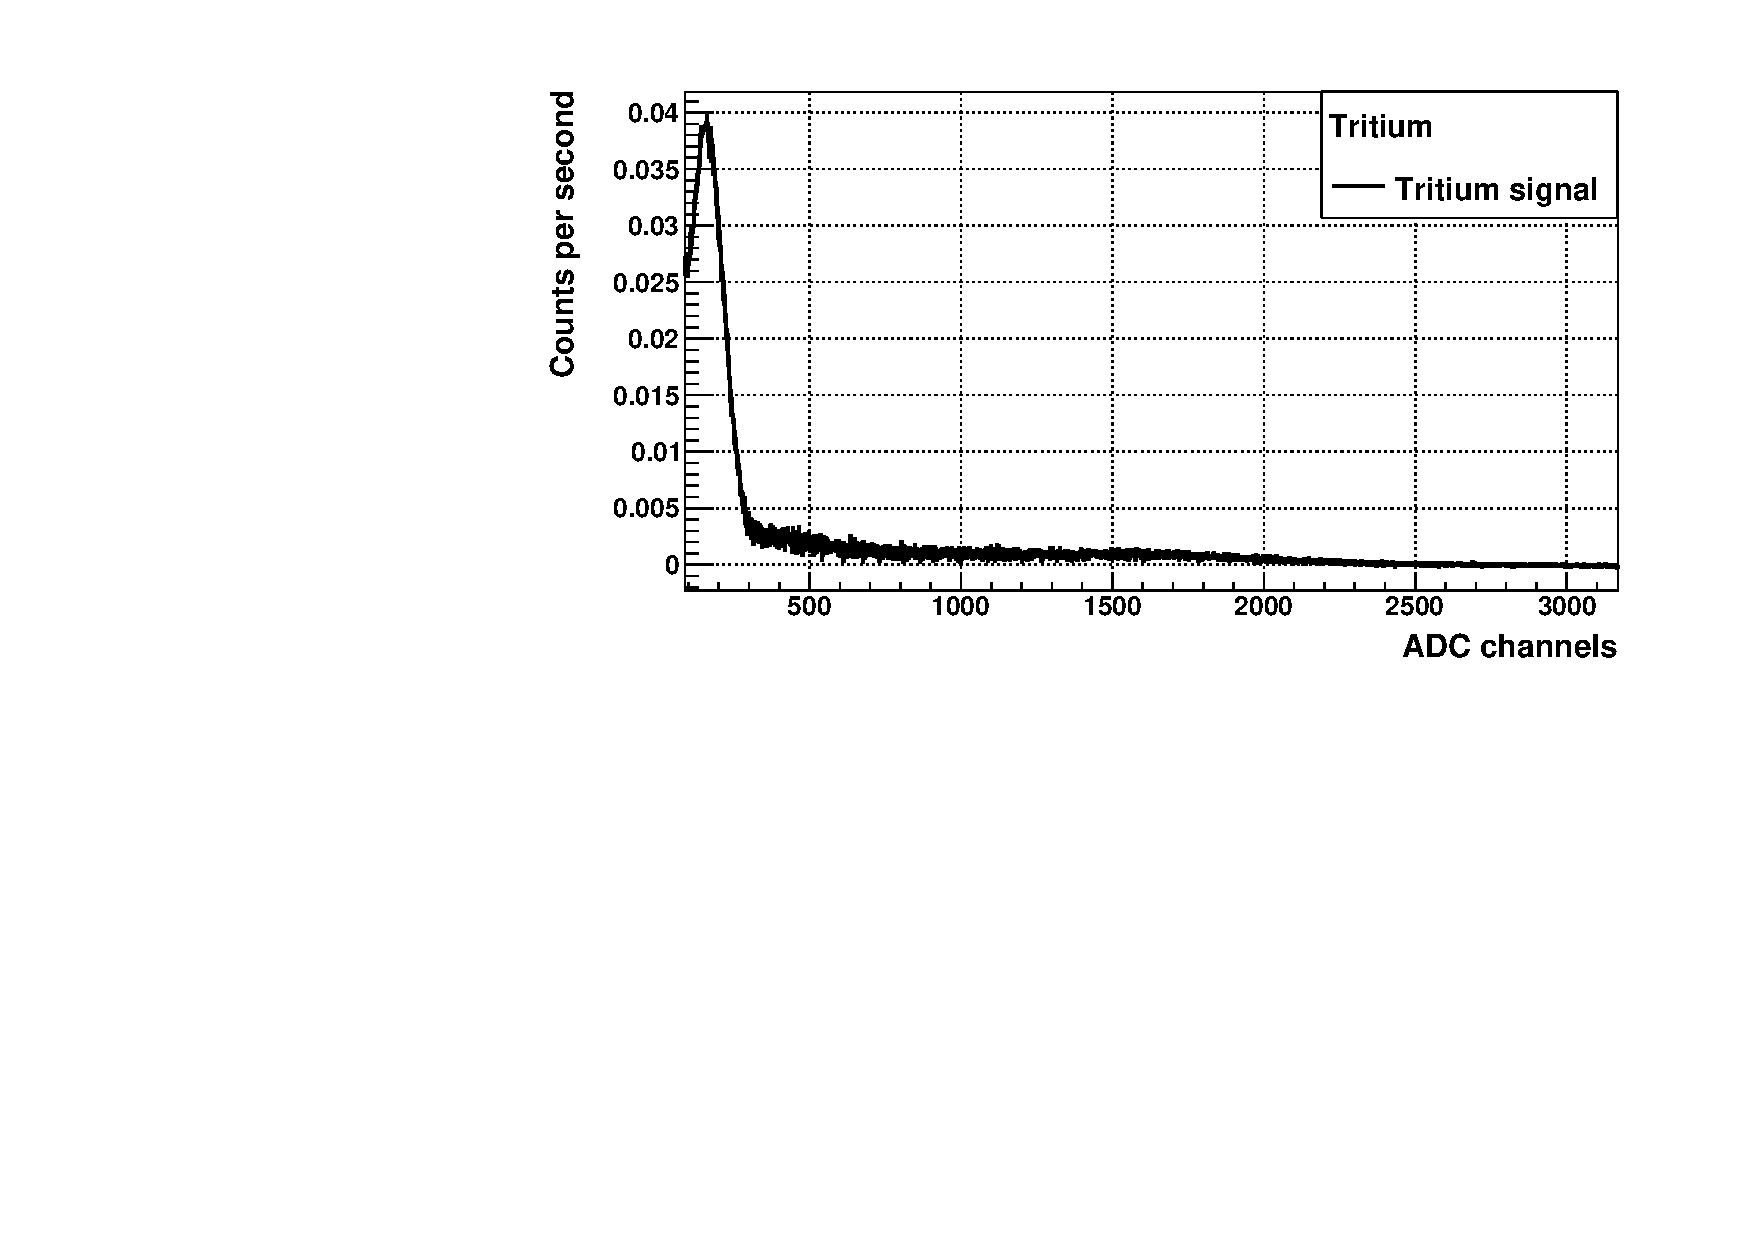
\includegraphics[width=\textwidth]{5Prototypes/53FinalPrototypes/532TritiumIFIC2/TritiumIFIC2ClearHigherZOOM_NP.pdf}  
    \caption{\label{subfig:TritiumEnergySpectraTritiumIFIC2}}
    \end{subfigure}
 \caption{Energy spectra measured with TRITIUM-IFIC-2. a) Signal and background energy spectra. b) Tritium energy spectrum.}
 \label{fig:EnergySpectraTRITIUMIFIC2}
\end{figure}

\begin{table}[htbp]
\centering{}%
\begin{tabular}{cc}
\toprule 
Spectrum & Rate (Hz) \tabularnewline
\midrule
\midrule 
Signal & $19.05 \pm 0.18$ \tabularnewline
Background & $11.54 \pm 0.14$ \tabularnewline  
Tritium & $7.11 \pm 0.23$ \tabularnewline
\bottomrule
\end{tabular}
\caption{Counting rates measured by TRITIUM-IFIC-2.}
\label{tab:CountsPerSecondTRITIUMIFIC2}
\end{table}
The tritium detection efficiency obtained for this prototype is $$\eta = (7.11 \pm 0.28)\cdot{} 10^{-1}~\liter\:\kilo\becquerel^{-1}\second^{-1}$$ 
This efficiency is larger than those reported in the literature (Table \ref{tab:PlasticScinTritium}). This is an expected result since the active area of this prototype is the largest. The specific efficiency is
$$S=(14.1 \pm 0.6)\cdot{} 10^{-5}~\liter\:\kilo\becquerel^{-1}\second^{-1}\cm^{-2}$$
which is the largest reported for tritium detection. 

A detector calibration in units of photons detected per event can be obtained from the single-photon distribution of the PMTs, shown in Figure \ref{fig:PhotonsPerTritiumEventIFIC2}. Fitting the single-photon distribution to a Gaussian function, the mean and uncertainty obtained are around $172$ and $66$ ADC channels, respectively, for one PMT and $173$ and $57$ ADC channels, respectively, for the other. The tritium rate given in number of photons detected per event is obtained as the ratio of the tritium energy spectrum and the single-photon distribution mean. A maximum of $15$ photons per tritium event is measured, which is in agreement with the results of the simulations described in Chapter \ref{chap:Simulations}. 
%The PMTs used to read this prototype was decoupled from the prototype and covered with a special black blanket to screen the PMT from external photons. 

\begin{figure}
\centering
    \begin{subfigure}[b]{0.9\textwidth}
    \centering
    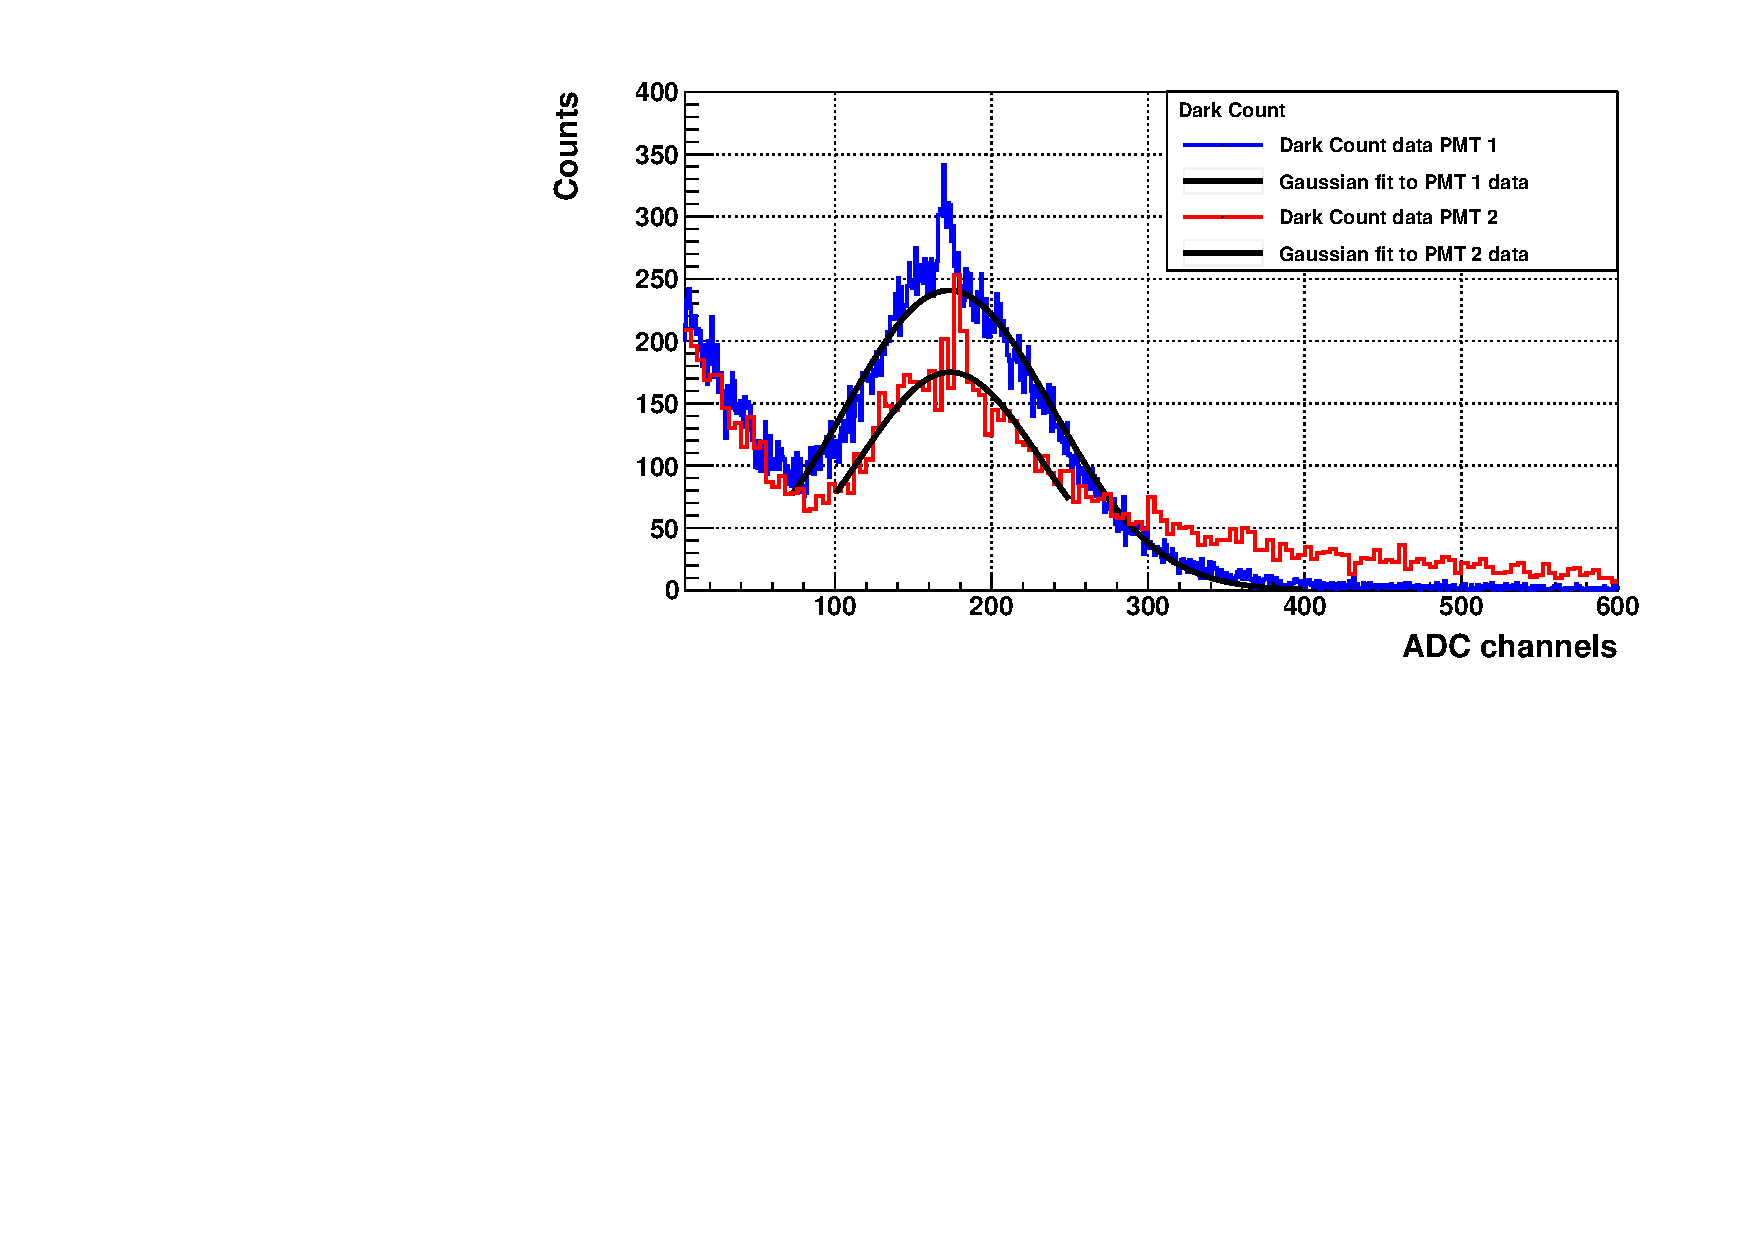
\includegraphics[width=\textwidth]{5Prototypes/53FinalPrototypes/532TritiumIFIC2/SinglePhotonDistribution2.pdf}  
    \caption{\label{subfig:SinglePhotonDistributionIFIC2}}
    \end{subfigure}
    \hfill
    \begin{subfigure}[b]{0.9\textwidth}
    \centering
    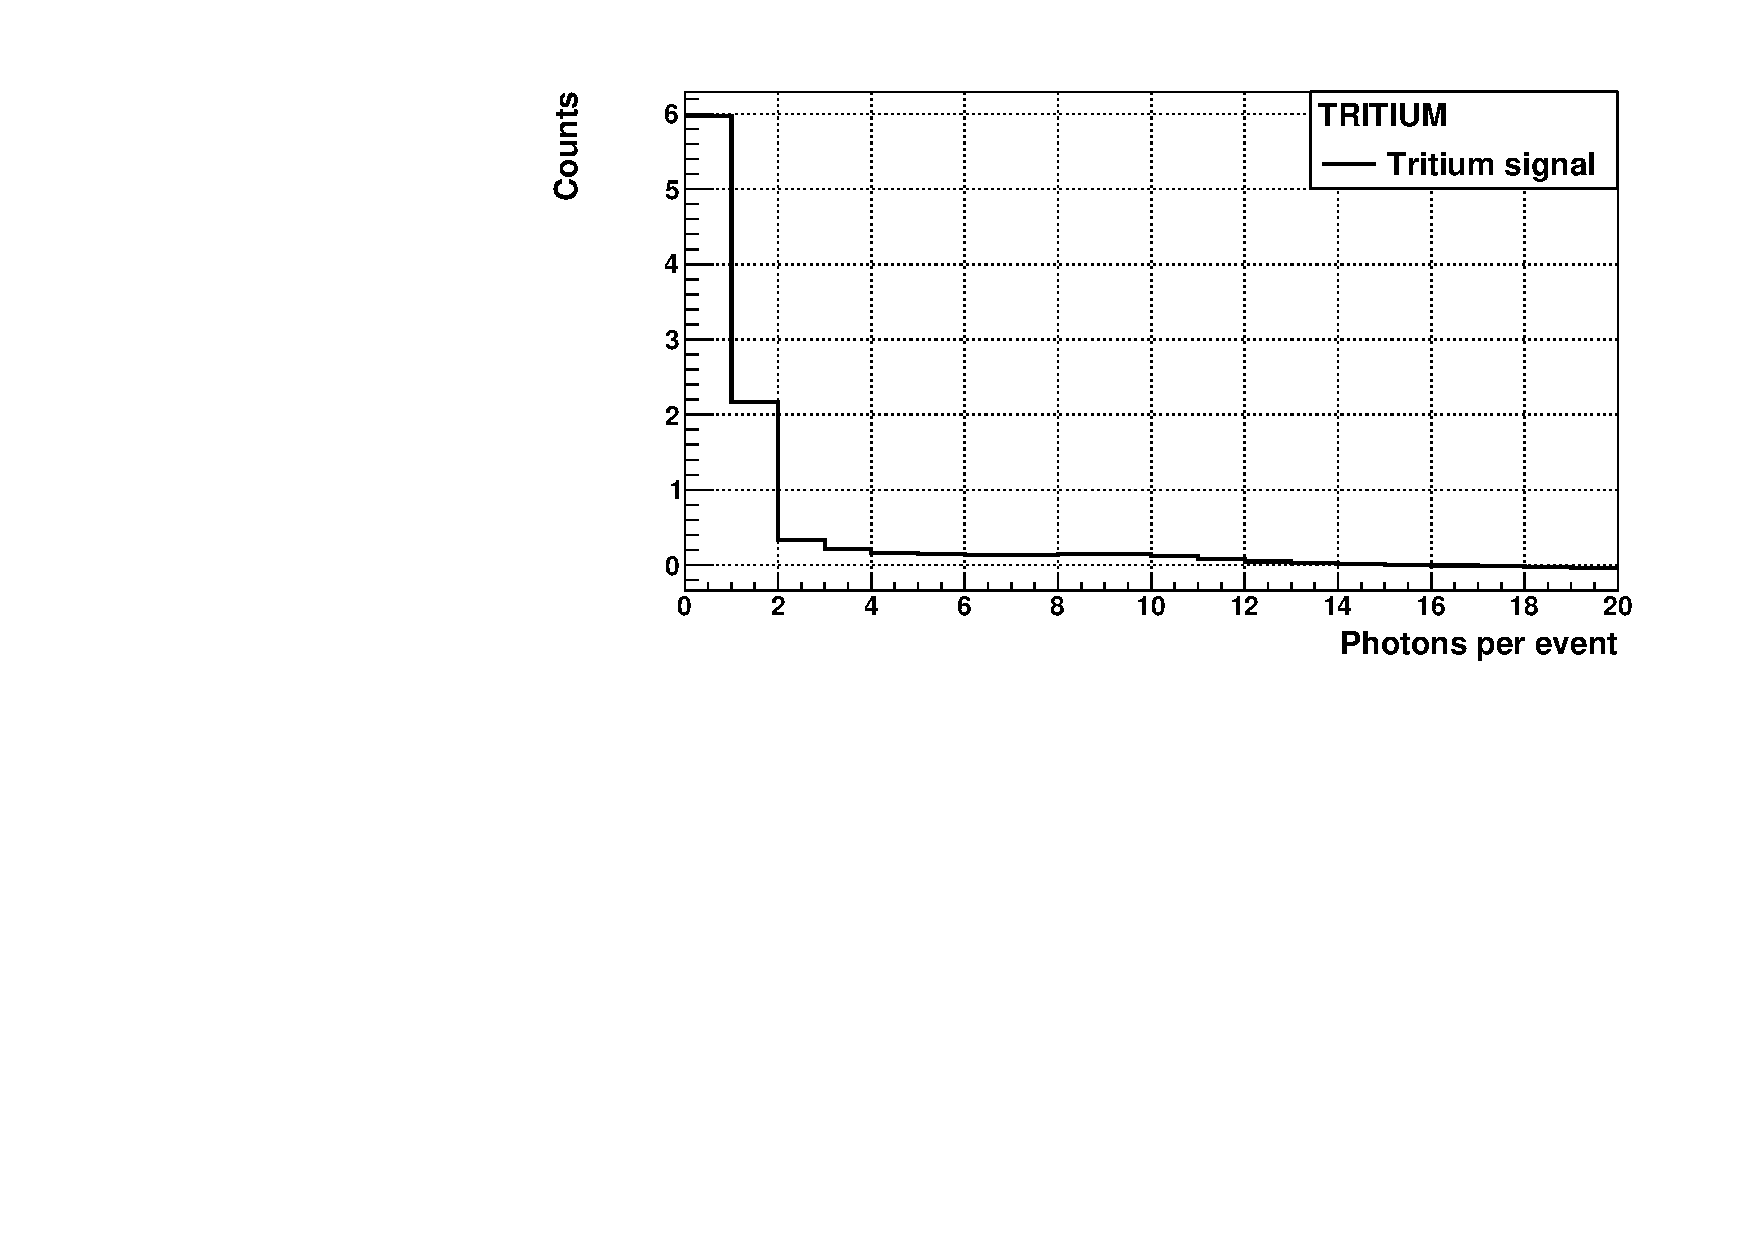
\includegraphics[width=\textwidth]{5Prototypes/53FinalPrototypes/532TritiumIFIC2/PhotonsPerTritiumEvent.pdf}  
    \caption{\label{subfig:TritiumSignalTRITIUMIFIC2}}
    \end{subfigure}
 \caption{a) Single photon distribution of TRITIUM-IFIC-2 PMTs. b) Tritium energy spectrum measured with TRITIUM-IFIC-2 versus number of photons detected per event.}
 \label{fig:PhotonsPerTritiumEventIFIC2}
\end{figure}

%\begin{figure}[h]
%\centering
%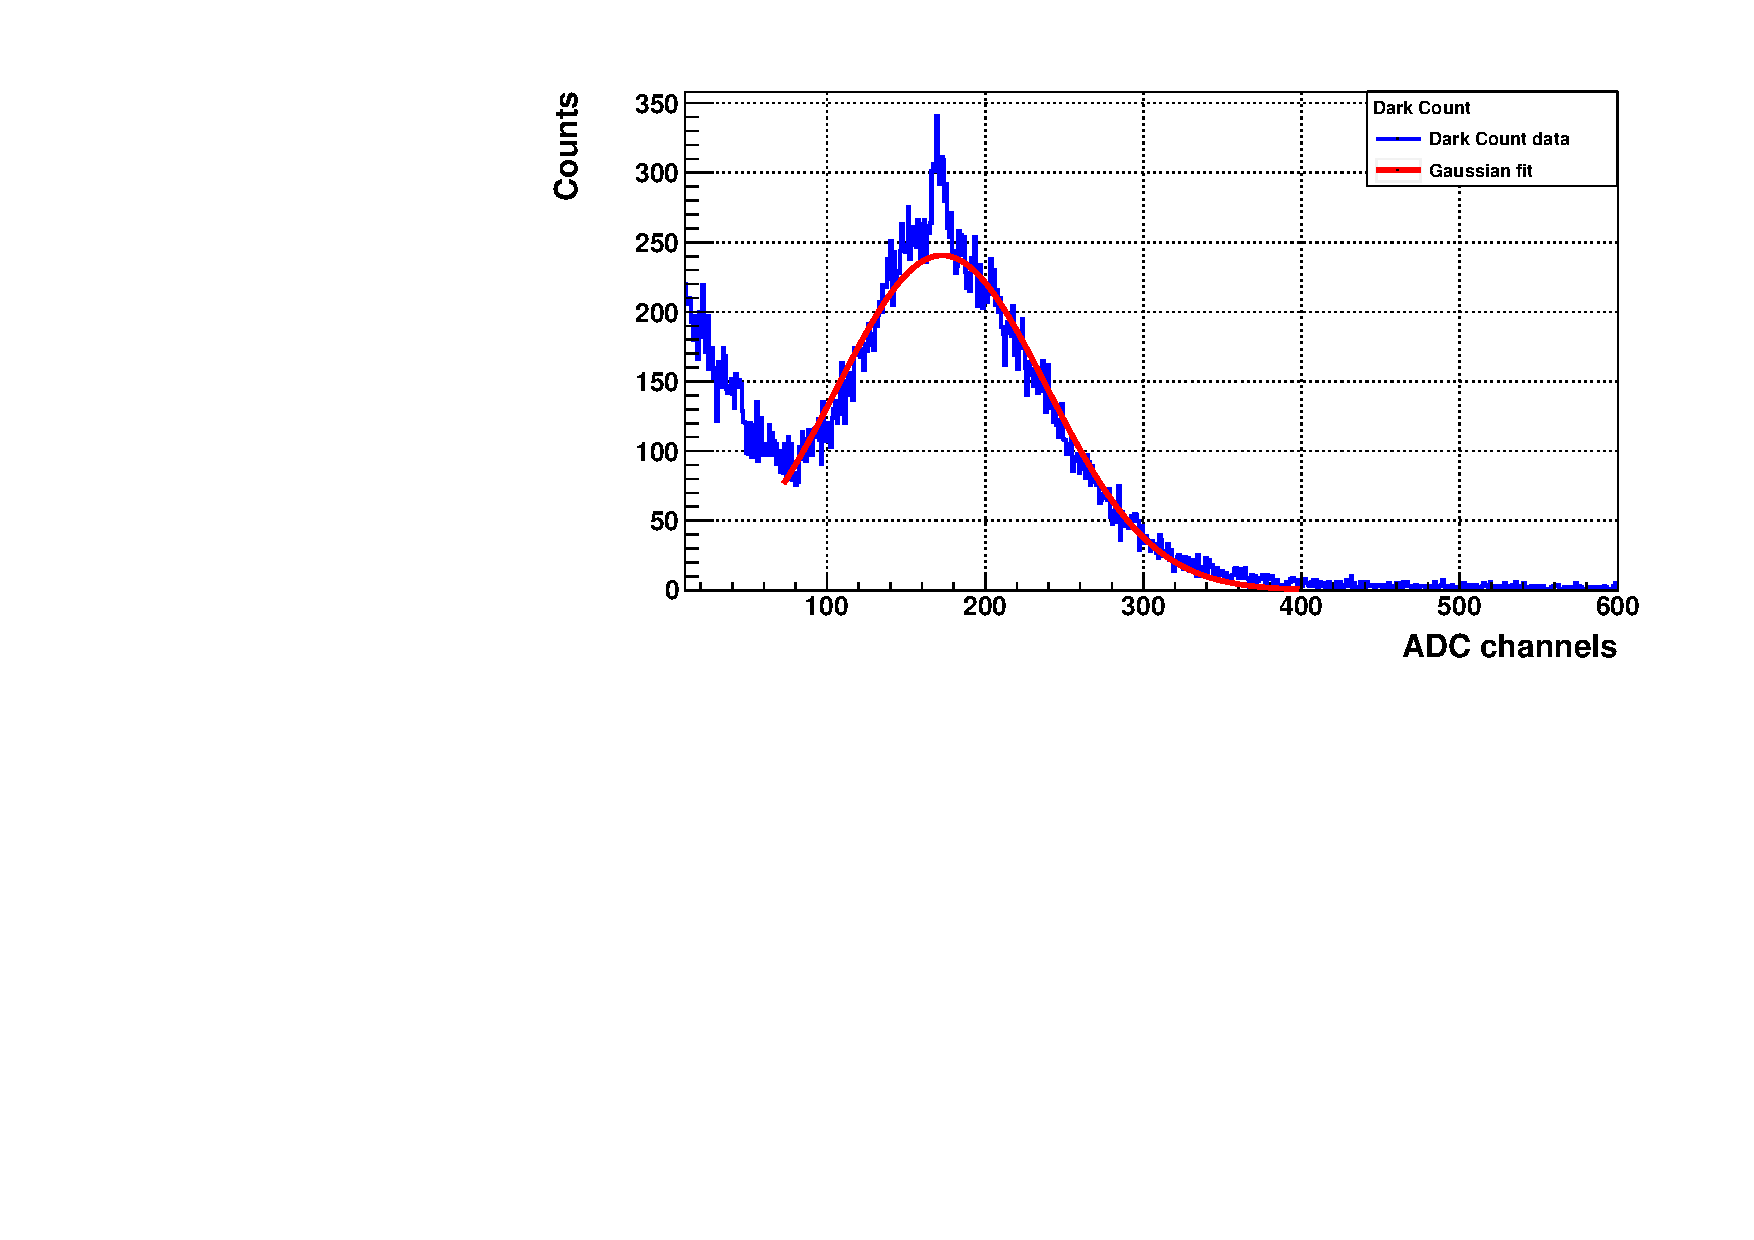
\includegraphics[scale=0.6]{5Prototypes/53FinalPrototypes/532TritiumIFIC2/SinglePhotonDistribution.pdf}
%\caption{Single photon energy distribution measured with the PMT used in TRITIUM-IFIC-2 prototype.\label{fig:SinglePhotonDistributionIFIC2}}
%\end{figure}

%\begin{figure}[h]
%\centering
%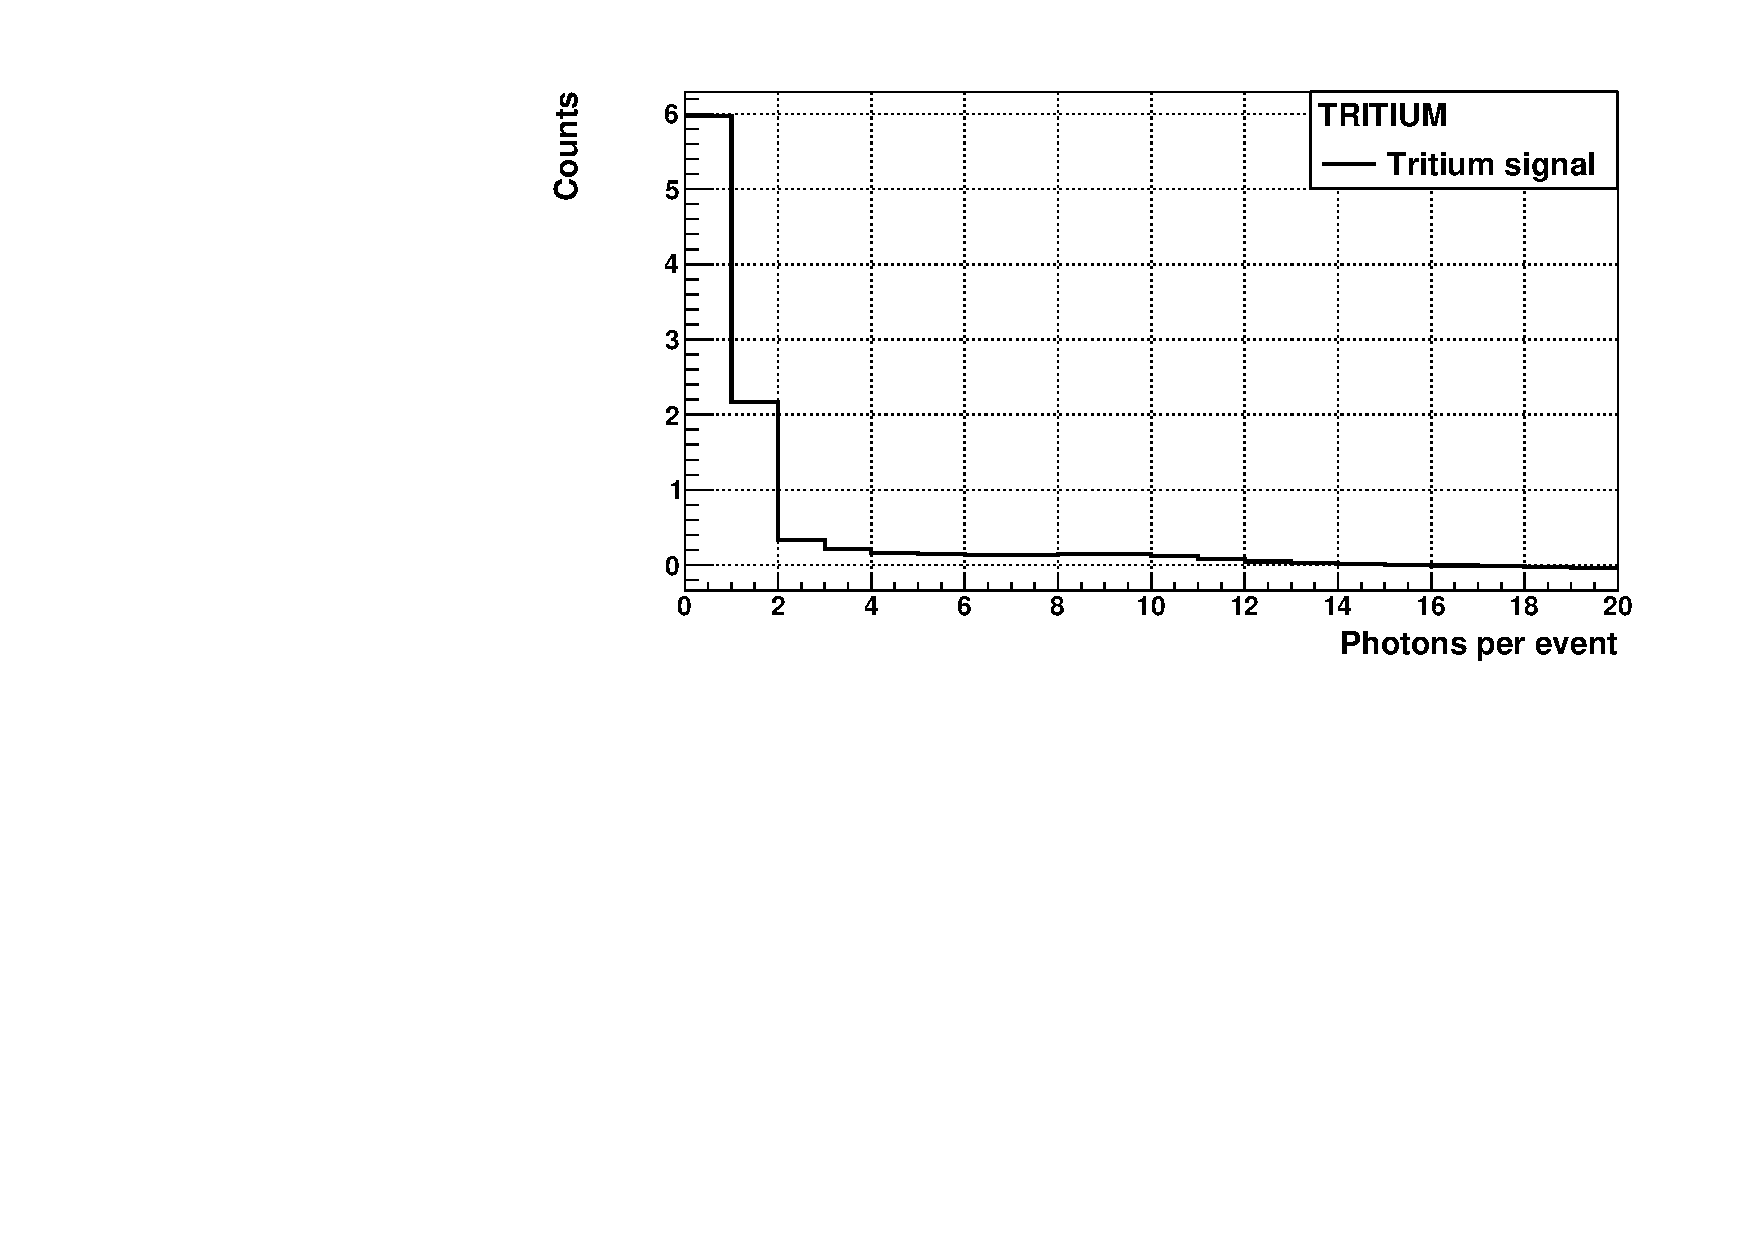
\includegraphics[scale=0.6]{5Prototypes/53FinalPrototypes/532TritiumIFIC2/PhotonsPerTritiumEvent.pdf}
%\caption{Tritium signal measured with the TRITIUM-IFIC-2 prototype and expressed in number of photones per tritium event detected.\label{fig:TritiumSignalTRITIUMIFIC2}}
%\end{figure}


%As can be seen, a maximum of $15$ photons are generated per tritium event, which corresponds to the best situation. To compare the value obtained with the expected one, the different energies and efficiencies involved are taken into account. Considering a maximum energy for the tritium electron detected, $18.6~\keV$, a scintillation yield of $8000~\text{ph}/\MeV$ for the fibres, a maximum collection efficiency for the fibres, $7\%/\meter$, the fibre length, $20~\cm$ (which increases the collection efficiency by a factor of 5), and the PMT efficiency, $29\%$, the maximum number of photons produced for a tritium event detected with TRITIUM-IFIC-2 prototype is $15$. As can be seen, this is perfectly in accordance with the measurement.

A monitoring of the signal and background prototypes was carried out during several months. The rates measured are shown in Figure \ref{fig:MonitorizationTRITIUMIFIC2}. No quenching of the signal with time was observed, which indicates the detector efficiency remained stable during about 6 months. A relative standard deviation of $2.5\%$ of the measured tritium rate was obtained.

\begin{figure}[h]
\centering
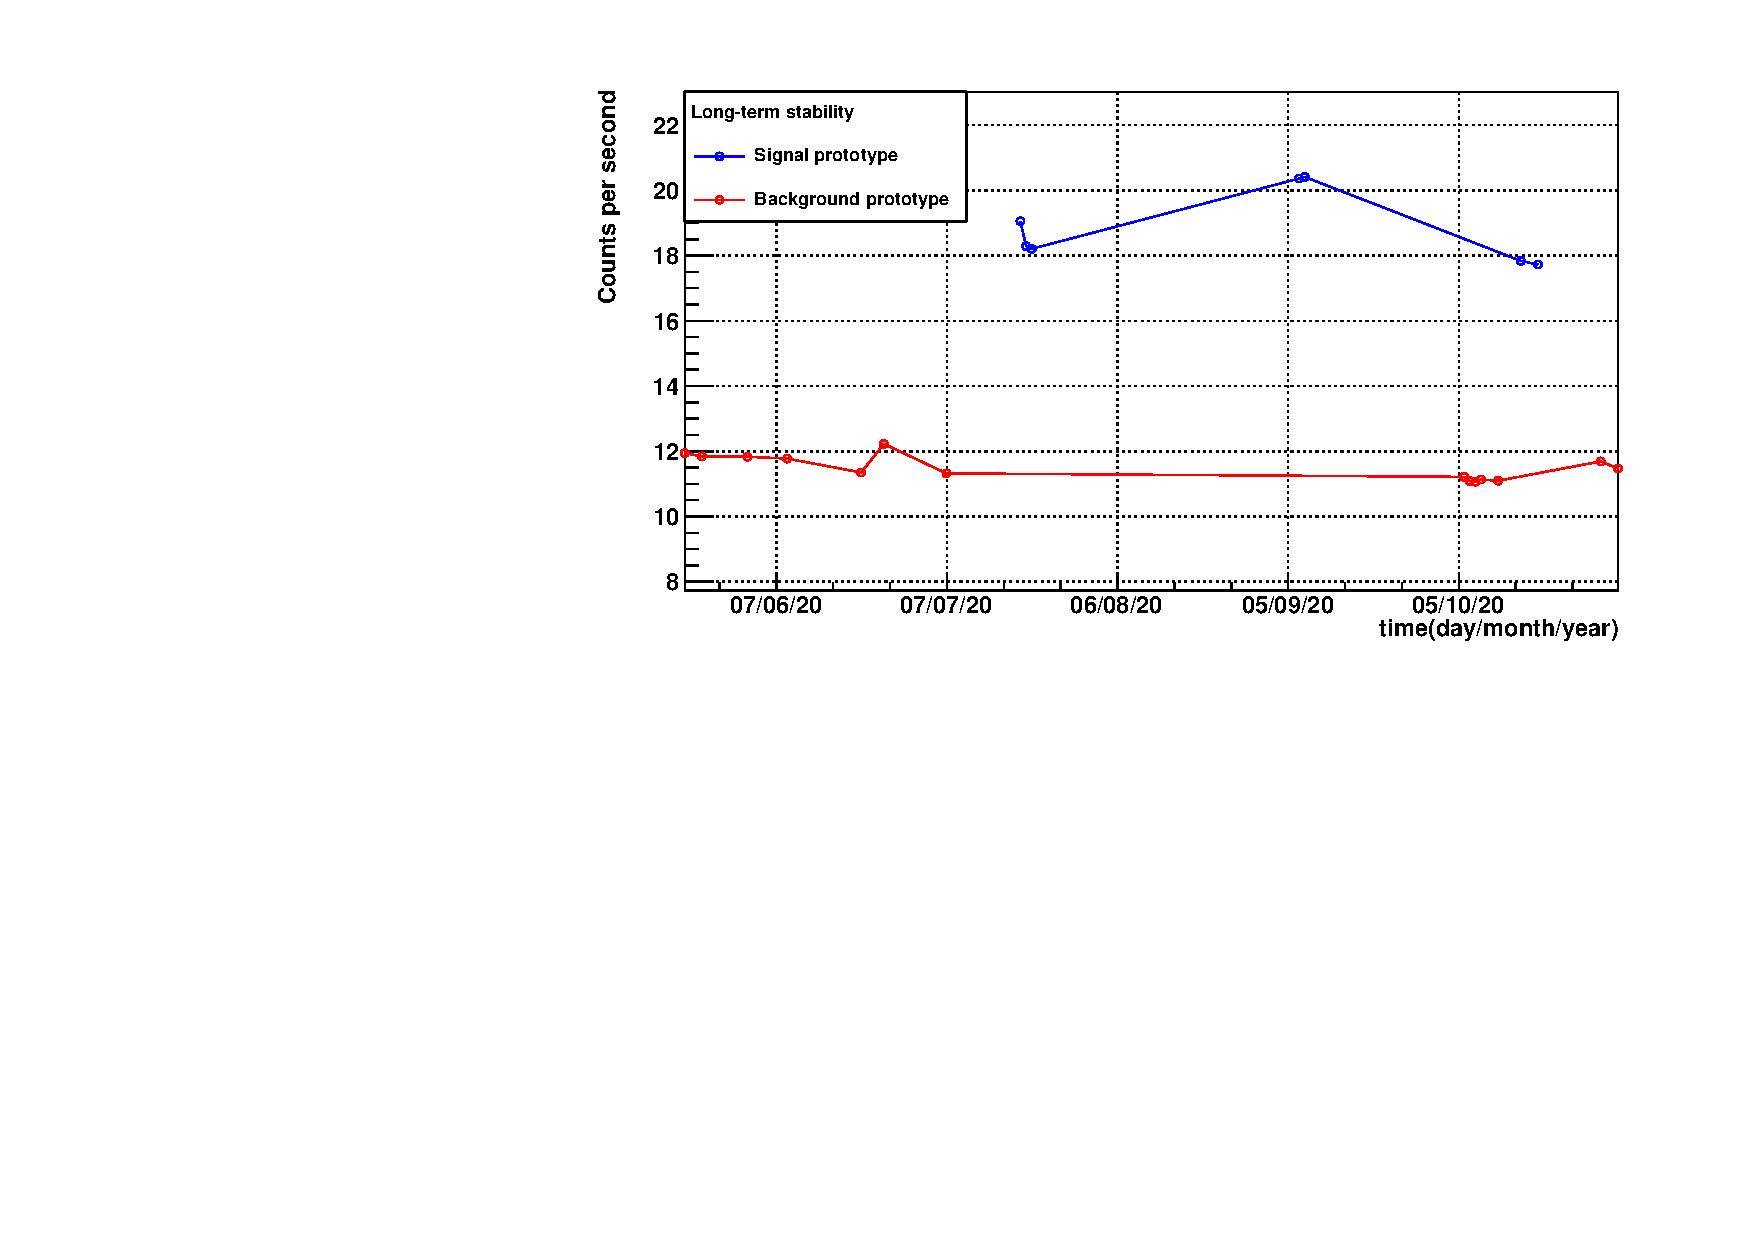
\includegraphics[scale=0.75]{5Prototypes/53FinalPrototypes/532TritiumIFIC2/Signal_Background_stability_ZOOM.pdf}
\caption{Signal and background rates for a long time measurement.\label{fig:MonitorizationTRITIUMIFIC2}}
\end{figure}

To calculate the MDA, the background was binned in $10~\min$ and $60~\min$ intervals. The mean values and standard deviation of these measurements are shown in the Table \ref{tab:CurrieLawTRITIUMIFIC2}. The $N_D$ and the $L_C$ obtained from the Currie criterium (Equation \ref{eq:EquationNetCounts}) are given in Table \ref{tab:CurrieLawTRITIUMIFIC2}.
\begin{table}[htbp]
\centering{}%
\begin{tabular}{ccccc}
\toprule 
Time (min.) & $N_b$ & $\sigma_{N_b}$ & $L_C$ & $N_D$ \tabularnewline
\midrule
\midrule 
$10$ & $5635$ & $82$ & $191$ & $384$ \tabularnewline
$60$ & $33969$ & $158$ & $368$ & $737$ \tabularnewline
\bottomrule
\end{tabular}
\caption{Mean value $\bar{N_b}$ and standard deviation $\sigma_{\bar{N_b}}$ of fourteen background measurements. $N_D$ and $L_C$ obtained from the Currie criterium.}
\label{tab:CurrieLawTRITIUMIFIC2}
\end{table}
The $N_D'$ referred to the detector signal before background subtraction are $6019$ and $34706$ for an integration time of $10~\min$ and $60~\min$, respectively. The MDA of tritium is obtained from $N_D'$ by associating the mean value of the background to a null tritium activity and the mean value of the signal to a tritium activity of $10~\kilo\becquerel/\liter$, assuming that counting rate scales linearly with activity. This results in an MDA of $677~\becquerel/\liter$ and $218~\becquerel/\liter$ for an integration time of $10~\min$ and $60~\min$, respectively. In addition, it has to be taken into account that one of the most important properties of the TRITIUM detector is scalability, which means that results can be improved by increasing the number of modules. The MDA of the TRITIUM monitor is expected to be reduced by the square root of the number of modules, according to equation \ref{eq:EquationNetCounts}. The plot of the MDA versus the number of modules is shown in Figure \ref{fig:MDATRITIUMmonitor}, where it can be seen that the goal of the TRITIUM project of measuring $100~\becquerel/\liter$ in quasi-real time is achieved with $45$ TRITIUM-IFIC-2 modules read out in parallel with an integration time of $10~\min$ or $5$ TRITIUM-IFIC-2 modules with an integration time of $1~\hour$, which is the cheaper and more realistic option. %Therefore, the cheaper and realistic option is to use $5$ TRITIUM-IFIC-2 read out in parallel with an integration time of $1~\hour$ 

\begin{figure}[h]
\centering
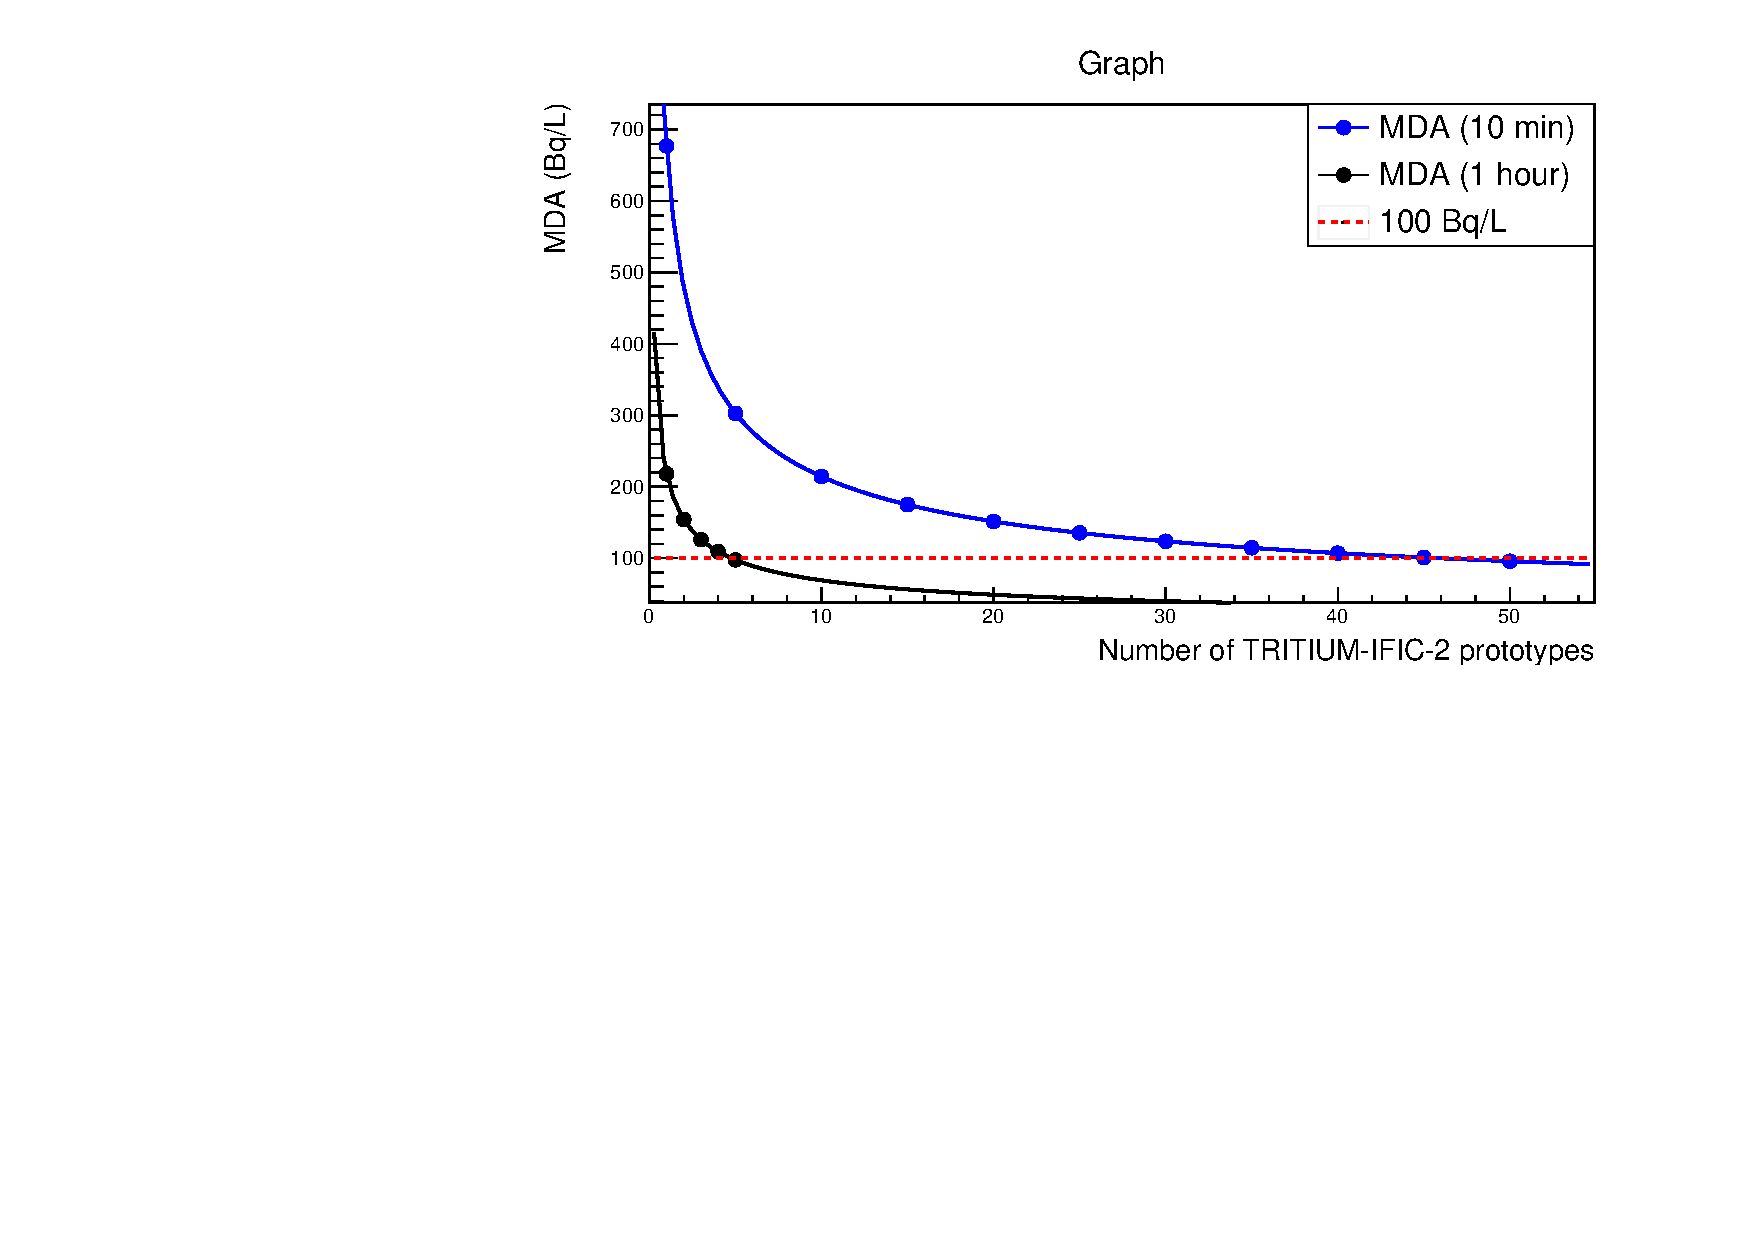
\includegraphics[scale=0.7]{5Prototypes/53FinalPrototypes/532TritiumIFIC2/MDA_1_hour_and_10_min_vs_N_Prototypes_logY.pdf}
\caption{MDA as a function of the number of TRITIUM-IFIC-2 modules read out in parallel for an integration time of $10~\min$ (blue line) and $1~\hour$ (black line). The dotted red line corresponds to $100~\becquerel/\liter$. \label{fig:MDATRITIUMmonitor}}
\end{figure}

%Medir en el prototipo con SIPM.

%As the sensitivity of the TRITIUM monitor scales with the number of TRITIUM modules used, the results obtained with the TRITIUM monitor should improve those results by a factor of $\sqrt{N}$, where N is the number of modules used.